  \documentclass{article}

%\geometry{showframe}% for debugging purposes -- displays the margins

\newcommand{\E}{\mbox{E}}
\newcommand{\MSE}{\mbox{MSE}}
\newcommand{\var}{\mbox{var}}
\newcommand{\bx}{\mathbf{x}}

\usepackage{amsmath}
%\usepackage[garamond]{mathdesign}
\usepackage{url}

% Set up the images/graphics package
\usepackage{graphicx}
\setkeys{Gin}{width=\linewidth,totalheight=\textheight,keepaspectratio}
\graphicspath{{graphics/}}

\title{Exercises 4: Hierarchical Models}
%\author[ ]{ }
\date{}  % if the \date{} command is left out, the current date will be used

% The following package makes prettier tables.  We're all about the bling!
\usepackage{booktabs}

% The units package provides nice, non-stacked fractions and better spacing
% for units.
\usepackage{units}

% The fancyvrb package lets us customize the formatting of verbatim
% environments.  We use a slightly smaller font.
\usepackage{fancyvrb}
\fvset{fontsize=\normalsize}

% Small sections of multiple columns
\usepackage{multicol}

% Provides paragraphs of dummy text
\usepackage{lipsum}

% These commands are used to pretty-print LaTeX commands
\newcommand{\doccmd}[1]{\texttt{\textbackslash#1}}% command name -- adds backslash automatically
\newcommand{\docopt}[1]{\ensuremath{\langle}\textrm{\textit{#1}}\ensuremath{\rangle}}% optional command argument
\newcommand{\docarg}[1]{\textrm{\textit{#1}}}% (required) command argument
\newenvironment{docspec}{\begin{quote}\noindent}{\end{quote}}% command specification environment
\newcommand{\docenv}[1]{\textsf{#1}}% environment name
\newcommand{\docpkg}[1]{\texttt{#1}}% package name
\newcommand{\doccls}[1]{\texttt{#1}}% document class name
\newcommand{\docclsopt}[1]{\texttt{#1}}% document class option name

\newcommand{\N}{\mbox{N}}
\newcommand{\thetahat}{\hat{\theta}}
\newcommand{\sigmahat}{\hat{\sigma}}
\newcommand{\betahat}{\hat{\beta}}


\begin{document}

\maketitle% this prints the handout title, author, and date


\section{Hierarchical models: data-analysis problems}

\subsection{Math tests}

The data set in ``mathtest.csv'' shows the scores on a standardized math test from a sample of 10th-grade students at 100 different U.S.~urban high schools, all having enrollment of at least 400 10th-grade students.  (A lot of educational research involves ``survey tests'' of this sort, with tests administered to all students being the rare exception.)

Let $\theta_i$ be the underlying mean test score for school $i$, and let $y_{ij}$ be the score for the $j$th student in school $i$.  Starting with the ``mathtest.R'' script, you'll notice that the extreme school-level averages $\bar{y}_i$ (both high and low) tend to be at schools where fewer students were sampled.

\begin{enumerate}
\item Explain briefly why this would be.
\item Fit a normal hierarchical model to these data via Gibbs sampling:
\begin{eqnarray*}
y_{ij} &\sim& \mbox{N}(\theta_i, \sigma^2) \\
\theta_i &\sim& \mbox{N}(\mu, \tau^2 \sigma^2)
\end{eqnarray*}
Decide upon sensible priors for the unknown model parameters $(\mu, \sigma^2, \tau^2)$.

\item Suppose you use the posterior mean $\hat{\theta}_i$ from the above model to estimate each school-level mean $\theta_i$.  Define the shrinkage coefficient $\kappa_i$ as
$$
\kappa_i = \frac{ \bar{y}_i - \hat{\theta}_i}{\bar{y}_i} \, ,
$$
which tells you how much the posterior mean shrinks the observed sample mean.  Plot this shrinkage coefficient (in absolute value) for each school as a function of that school's sample size, and comment.

\end{enumerate}

\textbf{Solution}
\begin{enumerate}
\item In schools with fewer students, the average scores will be more affected by outliers. In school with more students, outliers have less effect on the average score.
\item 
We assume a flat prior on \(\mu\), a Jeffreys prior on \(\sigma^2\) and an inverse Gamma prior on \(\tau^2\).
\begin{align*}
p(\sigma^2) &\propto 1/\sigma^2\\
p(\lambda)  &= \mbox{Gamma}(0.1, 0.1)
\end{align*}
where \(\lambda = 1 / \tau^2\).

(Update: the inverse Gamma prior is not well-behaved near \(0\), this may cause problems.)

To implement a Gibbs sampler, we need the conditional posterior of each variable. For \(\theta_i\), we have:
\begin{align*}
p(\theta_i \mid \mu, \tau, \sigma^2, y) = N(\hat{\theta_i}, 1/p_i)
\end{align*}
where:
\begin{align*}
p_i &= \frac{1}{\tau^2 \sigma^2} + \frac{n_i}{\sigma^2}\\
\hat{\theta}_i &= \left(\frac{\mu}{\tau^2 \sigma^2} + \frac{\bar{y}_i n_i}{\sigma^2}\right) \frac{1}{p_i}
\end{align*}
For \(\mu\), we have:
\begin{align*}
p(\mu \mid \theta, \tau, \sigma, y) &\propto p(\theta \mid \mu, \tau, \sigma, y)\\
%&= \prod_i N(\theta_i \mid \mu, \tau^2\sigma^2)\\
%&= N(\bar{\theta} \mid \mu, \tau^2\sigma^2/m )\\
&\propto N(\bar{\theta}, \frac{m}{\tau^2\sigma^2})
\end{align*}
where \(m\) is the number of groups.

For \(\sigma^2\), let \(t = 1/\sigma^2\). We have the precision prior: \(p(t) = 1/t\) and: 
\begin{align*}
p(t \mid \mu, \theta, \tau, y) &\propto p(t) p(\theta \mid t, \lambda)p(y \mid \sigma^2, \mu, \theta, \tau)\\
&\propto \frac{1}{t} \prod_i N(\theta_i \mid \mu, (t\lambda)^{-1}) \prod_j N(y_{ij} \mid \theta_i, t^{-1})\\
&\propto \frac{1}{t} \prod_i (t\lambda)^{1/2} \exp \left(-\frac{t\lambda(\theta_i - \mu)}{2} \right) \prod_j t^{1/2} \exp \left( -\frac{t(y_{ij} - \theta_i)^2}{2} \right)\\
&\propto t^{\frac{m + n}{2} - 1} \exp \left( -\frac{t \sum_i(\theta_i -\mu)^2 \sum_j (y_{ij} - \theta_i)^2}{2} \right)\\
&\propto \mbox{Gamma}\left((\frac{m+n}{2}, \frac{\sum_i(\theta_i -\mu)^2 \sum_j (y_{ij} - \theta_i)^2}{2}\right)
\end{align*}

For \(\tau^2\), we work with \(\lambda = 1/\tau^2\):
\begin{align*}
p(\lambda \mid t, \mu, \theta, y) &\propto p(\lambda) p(\theta \mid \lambda, t, \mu, y) \\
&\propto \mbox{Gamma}(\lambda \mid 0.1, 0.1) \prod_i N(\theta_i \mid \mu, (\lambda t) ^{-1})\\
&\propto \lambda^{0.1 - 1} \exp(-0.1\lambda) \prod_i (\lambda t)^{1/2} \exp \left( - \frac{\lambda t (\theta_i - \mu)^2}{2} \right)\\
&\propto \lambda^{0.1 + \frac{m}{2} - 1} \exp \left( -\frac{\lambda[0.2 + t\sum_i(\theta_i - \mu)^2]}{2}\right)\\
&\propto \mbox{Gamma}\left(0.1 + \frac{m}{2}, 0.1 + \frac{t\sum_i(\theta_i - \mu)^2}{2} \right)
\end{align*}

Code: mathtest.r

\item We can see that the shrinkage coefficient is large for schools with small sample sizes.
\begin{figure}[h]
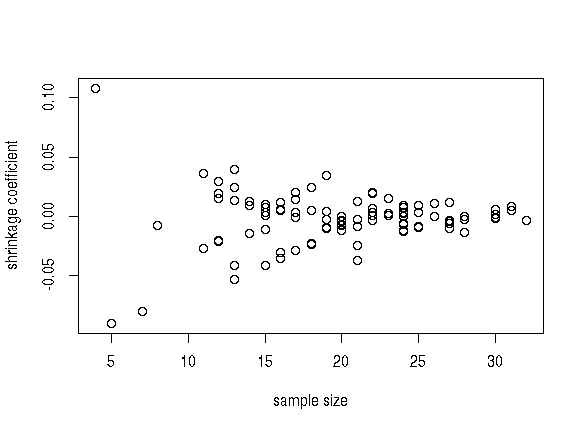
\includegraphics[width=\textwidth]{mathtest.jpeg}
\caption{Shrinkage coefficient against school sample size.}
\end{figure}

\end{enumerate}


\subsection{Price elasticity of demand}

The data in ``cheese.csv'' are about sales volume, price, and advertisting display activity for packages of Borden sliced ``cheese.'' The data are taken from Rossi, Allenby, and McCulloch's textbook on \textit{Bayesian Statistics and Marketing.} For each of 88 stores (store) in different US cities, we have repeated observations of the weekly sales volume (vol, in terms of packages sold), unit price (price), and whether the product was advertised with an in-store display during that week (disp = 1 for display).

Your goal is to estimate, on a store-by-store basis, the effect of display ads on the demand curve for cheese.  A standard form of a demand curve in economics is of the form $Q = \alpha P^\beta$, where $Q$ is quantity demanded (i.e.~sales volume), $P$ is price, and $\alpha$ and $\beta$ are parameters to be estimated.  You'll notice that this is linear on a log-log scale,
$$
\log P = \log \alpha + \beta \log Q \,
$$
which you should feel free to assume here.  Economists would refer to $\beta$ as the price elasticity of demand (PED).  Notice that on a log-log scale, the errors enter multiplicatively.

There are several things for you to consider in analyzing this data set.
\begin{itemize}
\item The demand curve might shift (different $\alpha$) and also change shape (different $\beta$) depending on whether there is a display ad or not in the store.
\item Different stores will have very different typical volumes, and your model should account for this.
\item Do different stores have different PEDs?  If so, do you really want to estimate a separate, unrelated $\beta$ for each store?
\item If there is an effect on the demand curve due to showing a display ad, does this effect differ store by store, or does it look relatively stable across stores?
\item Once you build the best model you can using the log-log specification, do see you any evidence of major model mis-fit?
\end{itemize}
Propose an appropriate hierarchical model that allows you to address these issues, and use Gibbs sampling to fit your model.

\textbf{Solution}
\begin{enumerate}
\item The model is:
\begin{align*}
\log (\mbox{vol}_i) = \alpha_{si} + \log (\mbox{price}_i) \cdot \beta_{si} + \mbox{disp}_i  \cdot \gamma_{si} + \epsilon_i 
\end{align*}
where \(i\) is the observation and \(si\) is the store for observation \(i\). Letting \(V, P\) and \(D\) be the log volume, log price and display, we have:
\begin{align*}
V_i = \alpha_{si} + P_i \cdot \beta_{si} + D_i  \cdot \gamma_{si} + \epsilon_i 
\end{align*}
The priors are:
\begin{align*}
\alpha_{si} \sim N(\mu_a, 1/t_a)\\
\beta_{si}  \sim N(\mu_b, 1/t_b)\\
\gamma_{si} \sim N(\mu_g, 1/t_g)\\
\end{align*}
We assume flat priors on \(\mu_a, \mu_b, \mu_g\) and \(t_a, t_b, t_g\).
Next, we derive the conditional distributions for Gibbs sampling. For \(\alpha\), we have:
\begin{align*}
p(\alpha_j | \ldots) &\propto \exp \left\lbrace -\frac{t}{2} \sum_{i, si = j} (\alpha_j + P_i \beta_j + D_i \gamma_j - V_i)^2 - \frac{t_a}{2} (\alpha_j - \mu_a)^2 \right\rbrace\\
&\propto \exp -\frac{1}{2}\left\lbrace \alpha_j^2(n_j t + t_a) - 2\alpha_jt \left[\sum_{i, si = j} (V_i - P_i \beta_j - D_i \gamma_j)  + t_a \mu_a\right] \right\rbrace\\
&\propto \exp -\frac{1}{2} \{ \alpha_j^2 A_j - 2 \alpha_j B_j \}\\
&\propto N\left(\frac{B_j}{A_j} , \frac{1}{A_j}\right)
\end{align*}
Where we let \(n_j\) be the number of observation in group \(j\), and \(A_j\) and \(B_j\) be the appropriate terms in the second line.

Similarly, for \(\beta\), we have:
\begin{align*}
p(\beta_j \mid \ldots) &\propto \exp -\frac{1}{2} \left\lbrace \beta_j^2(t \sum_i P_i^2 + t_b) - 2\beta_j \left[t\sum_i P_i(V_i - \alpha_j - D_i \gamma_j) + t_b \mu_b\right]  \right\rbrace\\
&\propto \exp -\frac{1}{2} \{ \beta_j^2 C_j - 2 \beta_j D_j \}\\
&\propto N\left(\frac{D_j}{C_j} , \frac{1}{C_j}\right)
\end{align*}
and for \(\gamma\), we have:
\begin{align*}
p(\gamma_j \mid \ldots) &\propto \exp -\frac{1}{2} \left\lbrace \gamma_j^2(t \sum_i P_i^2 + t_b) - 2\gamma_j \left[t\sum_i P_i(V_i - \alpha_j - P_i \beta_j) + t_g \mu_g\right]  \right\rbrace\\
&\propto \exp -\frac{1}{2} \{ \gamma_j^2 E_j - 2 \gamma_j F_j \}\\
&\propto N\left(\frac{F_j}{E_j} , \frac{1}{E_j}\right)
\end{align*}
For the prior mean \(\mu_a, \mu_b\) and \(\mu_g\), we have:
\begin{align*}
p(\mu_a \mid \ldots) &\propto \prod_j \exp \left\lbrace -\frac{t_a}{2} (\alpha_j - \mu_a)^2 \right\rbrace\\
&\propto N\left(\frac{\sum_j \alpha_j}{m}, (m t_a)^{-1}\right)
\end{align*}
(the equations for \(\mu_b\) and \(\mu_g\) are similar).

For the prior precision \(t_a, t_b\) and \(t_g\), we have:
\begin{align*}
p(t_a \mid \ldots) &\propto t_a^{m/2} \prod_j \exp \left\lbrace - \frac{t_a}{2} (\alpha_j - \mu_a)^2 \right\rbrace\\
&\propto \mbox{Gamma}\left(\frac{m}{2} + 1, \frac{1}{2} \sum_j (\alpha_j - \mu_a)^2\right)
\end{align*}
(the equations for \(t_b\) and \(t_g\) are similar).

\begin{figure}[h]
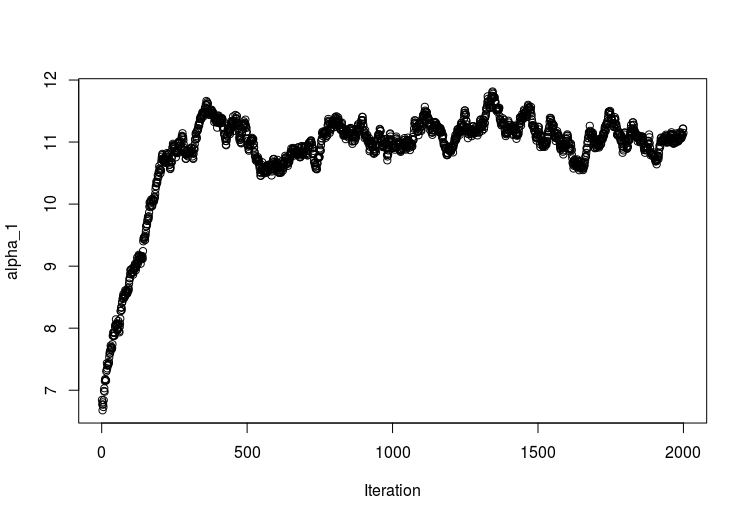
\includegraphics[width=\textwidth]{alpha1.jpeg}
\caption{The values of \(\alpha_1\) for all iterations, including a burn-in period in the beginning.}
\end{figure}


\begin{figure}[h]
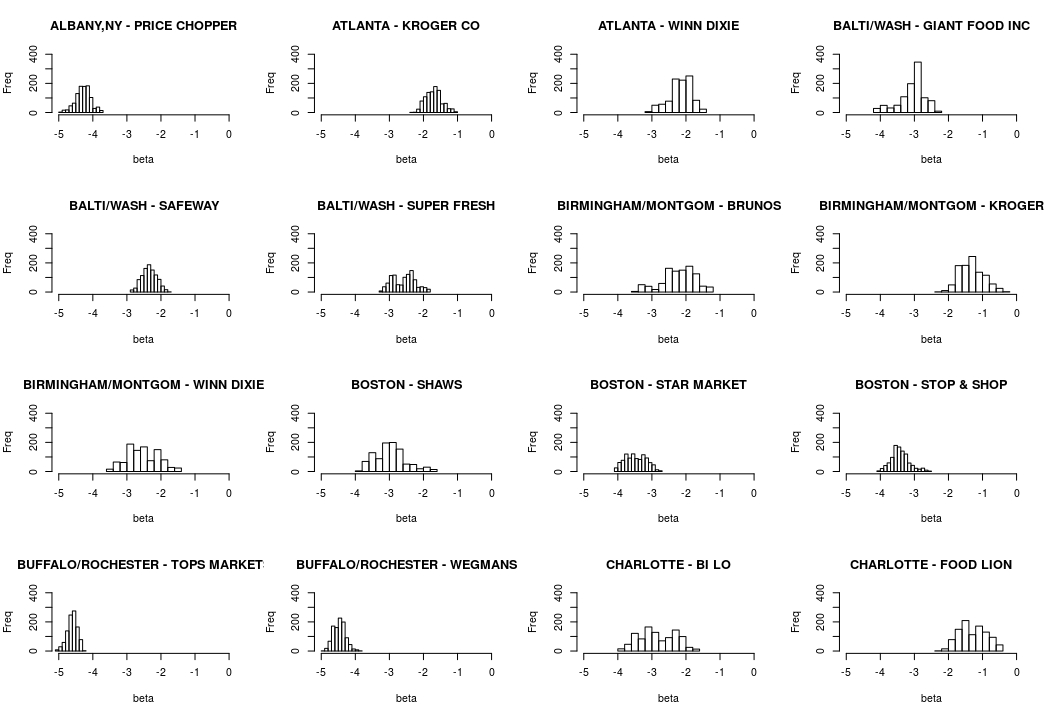
\includegraphics[width=\textwidth]{beta.jpeg}
\caption{Histograms of the elasticity for some stores.}
\end{figure}


\begin{figure}[h]
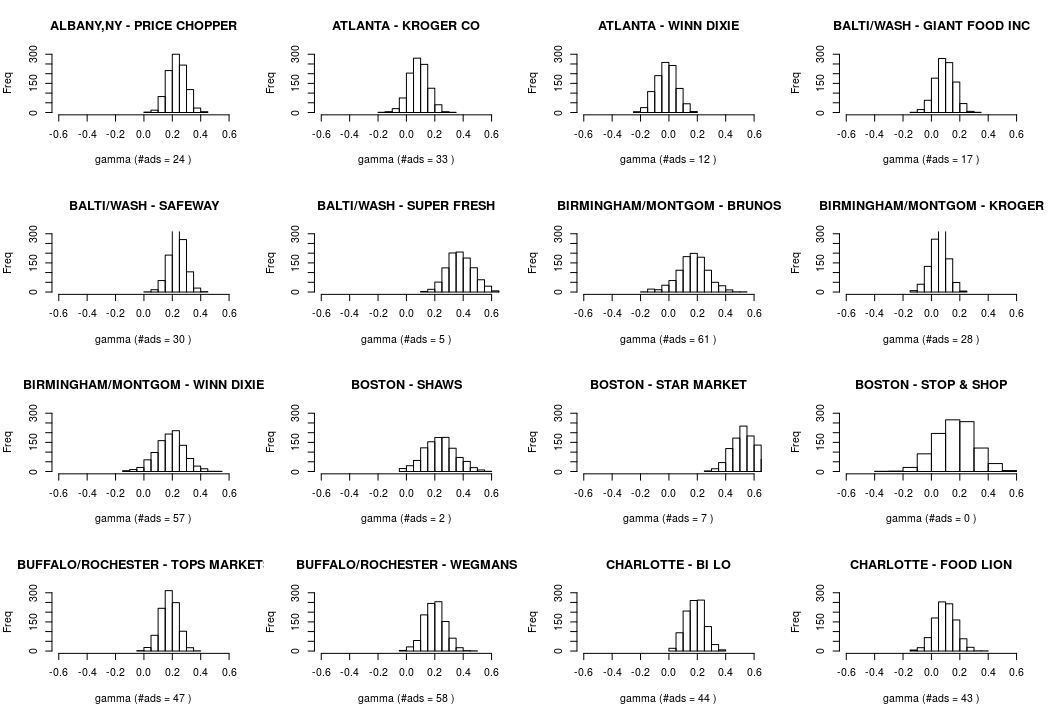
\includegraphics[width=\textwidth]{gamma.jpeg}
\caption{Histograms of the ad parameter for some stores.}
\end{figure}


\end{enumerate}

\subsection{A hierarchical probit model via data augmentation}

Read the following paper:
\begin{quotation}
``Bayesian Analysis of Binary and Polychotomous Response Data.''  James H. Albert and Siddhartha Chib.  \textit{Journal of the American Statistical Association}, Vol.~88, No.~422 (Jun.,~1993), pp.~669-679
\end{quotation}
The surefire way to get this paper is via access to JStor through the UT Library website.  Let me know if this is an issue for you.

The paper describes a Bayesian treatment of probit regression (similar to logistic regression) using the trick of \textit{data augmentation}---that is, introducing ``latent variables'' that turn a hard problem into a much easier one.  Briefly summarize your understanding of the key trick proposed by this paper.  Then see you if you can apply the trick in the following context, which is more complex than ordinary probit regression.

In ``polls.csv'' you will find the results of several political polls from the 1988 U.S.~presidential election.  The outcome of interest is whether someone plans to vote for George Bush (senior, not junior).  There are several potentially relevant demographic predictors here, including the respondent's state of residence.  The goal is to understand how these relate to the probability that someone will support Bush in the election.  You can imagine this information would help a great deal in poll re-weighting and aggregation (ala Nate Silver).

Use Gibbs sampling, together with the Albert and Chib trick, to fit a hierarchical probit model of the following form:
\begin{eqnarray*}
\mbox{Pr}(y_{ij} = 1) &=& \Phi(z_{ij})  \\
z_{ij} &=& \mu_i + x_{ij}^T \beta_i \, .
\end{eqnarray*}
Here $y_{ij}$ is the response (Bush=1, other=0) for respondent $j$ in state $i$; $\Phi(\cdot)$ is the probit link function, i.e.~the CDF of the standard normal distribution; $\mu_i$ is a state-level intercept term; $x_{ij}$ is a vector of respondent-level demographic predictors; and $\beta_i$ is a vector of regression coefficients for state $i$.

Notes:
\begin{enumerate}
\item There are severe imbalances among the states in terms of numbers of survey respondents. Following the last problem, the key is to impose a hierarchical prior on the state-level parameters.
\item The data-augmentation trick from the Albert and Chib paper above is explained in many standard references on Bayesian analysis.  If you want to get a quick introduction to the idea, you can consult one of these.  A good presentation is in Section 8.1.1 of ``Bayesian analysis for the social sciences'' by Simon Jackman, available as an ebook through lib.utexas.edu.
\item You are welcome to use the logit model instead of the probit model.  If you do this, you'll need to read the following paper, rather than Albert and Chib: Polson, N.G., Scott, J.G. and Windle, J. (2013). Bayesian inference for logistic models using Polya-Gamma latent variables. J. Amer. Statist. Assoc. 108 1339--1349.  
\end{enumerate}


\subsection{Gene expression over time}

In \verb|droslong.csv|, you will find a small subset of a time-course DNA microarray experiment.  The gene-expression profiles of 2000 different genes in the fruit fly (Drosophila) genome are tracked over time during embryogenesis; you are getting data on 14 of these genes, organized in three groups (think of these as marking which cellular pathway that gene influences).  For each gene at each time point, there are 3 ``technical replicates''---that is, three copies of the same biological material from the same fly, run through the same process to measure gene expression.

The question of interest is: how does each gene's expression profile change over time, as the process of embryogenesis unfolds?  Propose a hierarchical model for this data that properly reflects its structure.  Fit this model using Gibbs sampling.

A nice graphics package is the ``lattice'' library.  Install and load this; then try commands such as
\begin{verbatim}
xyplot(log2exp~time | gene, data=droslong)
xyplot(log2exp~time | group, data=droslong)
\end{verbatim}
to begin exploring the structure of this data.  If you know ggplot2, you can easily accomplish similar things.


\end{document}

